\documentclass[12pt,letterpaper,doublespaced,ETD]{gt-ece-thesis}
\usepackage{color}
\usepackage{graphicx}
\definecolor{darkgreen}{rgb}{0,0.5,0}
\newcommand{\Ntrg}{\big[N_{t=1, m=1} + \lambda \big] + \big[N_{t=1, m=2} + \lambda \big] + \ldots + \big[N_{t=1, m=M} + \lambda \big]}
\newcommand{\jointcnt}{\sum\limits_{n_{trg}=1}^{N_{trg}}I(X_t=x_t, X_{t-1}=x_{t-1})}
\newcommand{\singlecnt}{\sum\limits_{n_{trg}=1}^{N_{trg}}I(X_{t-1}=x_{t-1})}
\newcommand{\singlep}{p(X_{t-1}=x_{t-1})}
\newcommand{\singlepone}{p(X_{t-1}=1)}
\newcommand{\singleptwo}{p(X_{t-1}=2)}
\newcommand{\singlepM}{p(X_{t-1}=M)}
\newcommand{\condp}{p(X_t=x_t | X_{t-1}=x_{t-1})}
\newcommand{\jointp}{p(X_t=x_t, X_{t-1}=x_{t-1})}
\newcommand{\KmeansOuterSum}{\sum\limits_{k=1}^K}
\newcommand{\KmeansInnerSum}{\sum\limits_{{i=1 \atop x_i \in \mathcal{K}_k}}^N}
\newcommand{\KmeansSum}{\KmeansOuterSum \KmeansInnerSum}
\newcommand{\RVQInnerSum}{\sum\limits_{{i=1 \atop g_i \mapsto m_{\tau, s}}}^N}
\newcommand{\RVQOuterSum}{\sum_{s=1}^S}
\newcommand{\RVQsum}{\KmeansOuterSum \sum\limits_{{i=1 \atop g_i \in \mathcal{K}_k}}^N}
\newcommand{\KmeansInner}{{(x_i - \mu_k)}^2}
\newcommand{\RVQinner}{            {(x_i  - \hat{\mu}^{(k)})}^2}
\newcommand{\RVQinneralternate}{{(g_i - m_\tau^{(k)})}^2}
\newcommand{\RVQinneralternatealternate}{{(g_i - m_{\tau, s})}^2}
\newcommand{\KmeansError}{\KmeansSum \KmeansInner}
\newcommand{\RVQerror}     {\KmeansSum \RVQinner}
\newcommand{\RVQerroralternate}{\RVQsum \RVQinneralternate}
\newcommand{\RVQunit}{x_i -\bigg(\sum_{t=1}^Tm^{(k)}_t\bigg)}
\newcommand{\RVQequivalentCodevector}{\sum_{t=1 }^Tm^{(k)}_t}
\newcommand{\RVQequivalentCodevectorBroken}{\sum_{t=1 \atop t \neq \tau}^Tm^{(k)}_t+ m^{(k)}_\tau}
\newcommand{\RVQmultipleKmeans}{x_i -\bigg(\RVQequivalentCodevectorBroken\bigg)}
\newcommand{\RVQmultipleKmeansone}{x_i -\sum_{t=2}^Tm^{(k)}_t+ m^{(k)}_1\bigg)}
\newcommand{\RVQmultipleKmeansonealternate}{\bigg(x_i -\sum_{t=1 \atop t \neq \tau}^Tm^{(k)}_t\bigg) - m^{(k)}_\tau}
\newcommand{\RVQmultipleKmeanstwo}{x_i -\bigg(\sum_{t=1 \atop t \neq 2}^Tm^{(k)}_t+ m^{(k)}_2\bigg)}
\newcommand{\RVQmultipleKmeansT}{x_i -\bigg(\sum_{t=1}^{T-1}m^{(k)}_t+ m^{(k)}_2\bigg)}
\newcommand{\EucMatrix}
{
\left[
\begin{array}{lll}
r_{11} & r_{12} & t_x \\ 
r_{21} & r_{22} & t_y \\ 
0 & 0 & 1 \\ 
\end{array}
\right]
}	

\newcommand{\SimMatrix}
{
\left[
\begin{array}{lll}
sr_{11} & sr_{12} & t_x \\ 
sr_{21} & sr_{22} & t_y \\
0 & 0 & 1 \\ 
\end{array}
\right]
}

\newcommand{\AffMatrix}
{
\left[
\begin{array}{lll}
a &b & t_x \\ 
c & d & t_y \\
0 & 0 & 1 \\
\end{array}
\right]
}

\newcommand{\ProjMatrix}
{
\left[
\begin{array}{lll}
h_{11} & h_{12} & h_{13} \\ 
h_{21} & h_{22} & h_{23} \\ 
h_{31} & h_{32} & h_{33} \\ 
\end{array}
\right]
}

\newcommand{\RotMatrixTheta}
{
\left[
\begin{array}{rr}
\cos(\theta) & -\sin(\theta) \\ 
\sin(\theta) & \cos(\theta) \\ 
\end{array}
\right]
}

\newcommand{\RotMatrixPhi}
{
\left[
\begin{array}{rr}
\cos(\phi) & -\sin(\phi) \\ 
\sin(\phi) & \cos(\phi) \\ 
\end{array}
\right]
}

\newcommand{\RotMatrixminusPhi}
{
\left[
\begin{array}{rr}
\cos(-\phi) & -\sin(-\phi) \\ 
\sin(-\phi) & \cos(-\phi) \\ 
\end{array}
\right]
}


\newcommand{\EigenvalueMatrix}
{
\left[
\begin{array}{cc}
\lambda_1 & 0\\
0 & \lambda_2
\end{array}
\right]
}

\newcommand{\bigMatrix}
{
s \left[
\begin{array}{cc}
 (r)(a) + b &  (r)(d) - c \\
 (r)(c) - d &  (r)(b) + a
\end{array}
\right]
}


\newcommand{\bigMatrixTwo}
{
\left[
\begin{array}{cc}
(\lambda_2) p + (\lambda_1) q & (\lambda_2) s  - (\lambda_1) r \\
(\lambda_2) r  - (\lambda_1) s & (\lambda_2) q + (\lambda_1) p
\end{array}
\right]
}
\newcommand{\dr}{(\mathbf{x}_i-\boldsymbol\mu_k)^T(\mathbf{x}_i-\boldsymbol\mu_k) + \lambda({Q_{\textrm{max}}-Q_i})}

\begin{document}






%#################################
\section{Stage subspaces}
%#################################
Figure~\ref{fig:Figure1} shows a simple example of a 2x2 RVQ with 4 input data points.  The error is given by

\begin{figure}
\center
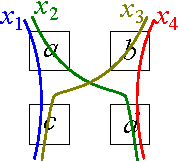
\includegraphics[width=0.5\textwidth]{thesis2/RVQ_CAC_toyExample2_2x2.pdf}
\caption{2x2 RVQ example}
\label{fig:Figure1}
\end{figure}

\begin{equation}
\begin{array}{lllll}
e &=& \KmeansError \\
&=& {(x_1 - a - c)}^2 + {(x_2- a - d)}^2 + {(x_3 - b - c)}^2 + {(x_4 - b - d)}^2\\
&=& {e_1}^2 + {e_2}^2 + {e_3}^2 + {e_4}^2
\end{array}
\end{equation}

Applying the CAC condition to optimize stage 1, we get the following equations by grouping all input data points with stage codevectors that do not belong to stage 1,

\begin{equation}
\begin{array}{lllll}
e &=& {((x_1 - c) - a)}^2 + {((x_2- d) - a)}^2 + {((x_3 - c) - b)}^2 + {((x_4 - d) - b)}^2
\end{array}
\label{Eqn:2x2RVQ_stage1}
\end{equation}

And similarly, to optimize stage 2, we get,

\begin{equation}
\begin{array}{lllll}
e &=& {((x_1 - a) - c)}^2 + {((x_2- a) - d)}^2 + {((x_3 - b) - c)}^2 + {((x_4 - b) - d)}^2
\end{array}
\label{Eqn:2x2RVQ_stage2}
\end{equation}

which leads to the optimal stage codevectors,

\begin{equation}
\begin{array}{lllll}
a = \frac{(x_1 - c) + (x_2 - d)}{2}\\
b = \frac{(x_3 - c) + (x_4 - d)}{2}\\
c = \frac{(x_1 - a) + (x_3 - b)}{2}\\
d = \frac{(x_2 - a) + (x_4 - b)}{2}\\
\end{array}
\end{equation}

Our next goal is to see if any relationship can be established between the subspace spanned by stage codevectors $a$ and $b$ and the subspace spanned by stage codevectors $c$ and $d$.
We can rewrite Equation~\ref{Eqn:2x2RVQ_stage1} as follows,

\begin{equation}
\begin{array}{lllll}
e &=& {((x_1 - a - c) + a - a)}^2 + {((x_2- a - d) + a - a)}^2 + {((x_3 - b - c) + b - b)}^2 + {((x_4 - b - d) + b - b)}^2 \\
 &=& {((e_1 + a) - a)}^2 + {((e_2 + a) - a)}^2 + {((e_3 + b) - b)}^2 + {((e_4 + b) - b)}^2 \\
\end{array}
\end{equation}

According to Ding and He, the above equation can be interpreted to mean that stage codevectors $a$ and $b$ should lie in the subspace spanned by $e_1+a$, $e_2+a$, $e_3 + b$ and $e_4 + b$.

Similary, Equation~\ref{Eqn:2x2RVQ_stage2} can be rewritten as follows,

\begin{equation}
\begin{array}{lllll}
e &=& {((x_1 - a - c) + c - c)}^2 + {((x_2- a - d) + d - d)}^2 + {((x_3 - b - c) + c - c)}^2 + {((x_4 - b - d) + d - d)}^2 \\
 &=& {(e_1 + c - c)}^2 + {(e_2 + d - d)}^2 + {(e_3 + c - c)}^2 + {(e_4 + d - d)}^2 \\
\end{array}
\end{equation}

And again, the above equation can be interpreted to mean that stage codevectors $c$ and $d$ lie in the subspace spanned by $e_1+c$, $e_2+d$, $e_3 + c$ and $e_4 + d$.  

To summarize, here are the steps:

\begin{enumerate}
\item The first step is to create an initial trellis.  Every stage codevector is computed from the K-means of residuals from the previous stage.  According to Ding and He, the codevectors at a stage lie in a subspace as determined by the principal components of inputs to that stage.  At this point, there appears to be no apparent relationship between the subspaces of the different stages.
\item At every iteration of CAC, we subtract from an input $x_i$, all stage codevectors that it maps to except for codevectors at stage $t$ that we're trying to optimize.  In other words, every single data point moves parallel to every subspace except the subspace in which those codevectors lie that we're trying to optimize.  In other words, the variance of the data changes causing the overall principal components as well as the stage principal components to rotate.
%\item We then find the stage codevectors for stage $t$.  The subspace in which these stage codevectors now lie in tilts towards all other subspaces since data has spread along those subspaces.
%\item Multiple iterations cause all subspaces to tilt towards each other.
%\item When we reach a minimum, all subspaces are aligned and we've recovered an M-dimensional manifold rather than an $M^T$ dimensional manifold.
\item At the global optimum, the stage subspace obtained by adding the error term $e_i$ (corresponding to each input data point $x_i$) to the stage codevector it corresponds to at that stage contains the stage codevectors at that stage.  In other words, instead of the initial data points $x_i$, consider the corresponding error terms $e_i$.  Now, if we want to find the subspace that is spanned by stage codevectors at a particular stage, take each data point $e_i$, find which codevectors at that stage $x_i$ maps to and add them to $e_i$.  This will create a new set of data points.  The required stage codevectors will lie in the subspace spanned by these new data points.
\end{enumerate}

The next question is, can we find a relation between the subspaces spanned by different stages.  The importance of this is that if there is such a relationship, then it may be easier to define a metric on codebook distance.



The optimal K means of the input data lie in the subspace spanned by the K-1 principal components of the input data.


%####################
\newpage
\section{Eigenspace Tracking}
%####################
In \cite{1998_JNL_Eigentracking_Black}, the authors use 200 images of Coke and 7-Up cans to create a linear PCA subspace.  They use the first 50 components.  Tracking is done using 


%####################################################################################################
\bibliographystyle{ieee}
\bibliography{c:/salman/work/writing/MyCitations}
\end{document}
%####################################################################################################
